\documentclass[a4paper]{jpconf}
\usepackage{graphicx}
\usepackage{color}
\usepackage{array}
\usepackage{enumerate}
\usepackage{cite}


\begin{document}
\title{The production deployment of IPv6 on WLCG}

\author{J Bernier$^1$, S Campana$^2$, K Chadwick$^3$, J Chudoba$^4$, 
        A Dewhurst$^5$, M Eli\'a\v s$^4$, S Fayer$^6$, T Finnern$^7$,
        C Grigoras$^2$, T~Hartmann$^8$, B Hoeft$^8$, T Idiculla$^5$, D P Kelsey$^5$,  
        F L\'opez Mu\~noz$^9$, E Macmahon$^{10}$, E Martelli$^2$, A P Millar$^7$, R Nandakumar$^5$, 
        K Ohrenberg$^7$, F Prelz$^{11}$, D Rand$^6$, 
        A Sciab\`a$^2$, U Tigerstedt$^{12}$, R Voicu$^{13}$, 
        C J Walker$^{14}$ and T Wildish$^{15}$}

\address{$^1$ IN2P3 Computing Center, 21 Avenue Pierre de Coubertin, F-69627 Villeurbanne Cedex, France}
\address{$^2$ CERN, CH-1211 Gen\`eve 23, Switzerland}
\address{$^3$ Fermi National Accelerator Laboratory, Batavia, Il 60510, U.S.A.}
%\address{$^3$ Institute of High Energy Physics, 19B Yuquanlu, Shijingshan District, 100049 Beijing, China} 
\address{$^4$ Institute of Physics, Academy of Sciences of the Czech Republic Na Slovance 2 182 21 Prague 8, Czech Republic}
\address{$^5$ STFC Rutherford Appleton Laboratory, Harwell Oxford, Didcot, Oxfordshire OX11 0QX, United Kingdom}
\address{$^6$ Imperial College London, South Kensington Campus, London SW7 2AZ, United Kingdom}
\address{$^7$ Deutsches Elektronen-Synchrotron, Notkestra\ss e 85, D-22607 Hamburg, Germany}
\address{$^8$ Karlsruher Institut f\"ur Technologie, Hermann-von-Helmholtz-Platz 1, D-76344 Eggenstein-Leopoldshafen, Germany}
\address{$^9$ Port d'Informaci\'o Cient\'ifica, Campus UAB, Edifici D, E-08193 Bellaterra, Spain}
\address{$^{10}$ The University of Oxford, The Department of Physics, Denys Wilkinson Building, Keble Road, Oxford OX1 3RH, United Kingdom}
\address{$^{11}$ INFN, Sezione di Milano, via G. Celoria 16, I-20133 Milano, Italy}
\address{$^{12}$ CSC Tieteen Tietotekniikan Keskus Oy, P.O. Box 405, FI-02101 Espoo, Finland}
\address{$^{13}$ California Institute of Technology, Pasadena, Ca 91125, U.S.A.}
\address{$^{14}$ Queen Mary University of London, Mile End Road, London E1 4NS, United Kingdom}
\address{$^{15}$ Princeton University, Jadwin Hall, Princeton, NJ 08544, U.S.A.}

\ead{david.kelsey@stfc.ac.uk, ipv6@hepix.org}

\begin{abstract}
The world is rapidly running out of IPv4 addresses; the number of IPv6 end systems connected
to the internet is increasing; WLCG and the LHC experiments may soon have access to worker
nodes and/or virtual machines (VMs) possessing only an IPv6 routable address. The HEPiX
IPv6 Working Group has been investigating, testing and
planning for dual-stack services on WLCG for several years. Following feedback from our
working group, many of the storage technologies in use on WLCG have recently been made
IPv6-capable.
This paper presents the IPv6 requirements, tests and plans of the LHC
experiments together with the tests performed on the group's IPv6 test-bed. 
This is primarily aimed at IPv6-only worker nodes or VMs
accessing several different implementations of a global dual-stack federated storage service.
Finally the plans for deployment of production dual-stack WLCG services are presented.
\end{abstract}

\section{Introduction}
blah blah


\section{Status and hurdles of the worldwide IPv4$\rightarrow$IPv6 transition}
We now offer a quick panorama of the IPv6 statistical trends since the last
CHEP conference and identify two factors that may be currently limiting 
the IPv6 adoption rate. 
\subsection{Survey of available statistical data}
An analysis of the available statistical data collected since 2013
by the Regional Internet Registries \cite{ripeipv6,arinstat,apnicstat,afrinicipv6,lacnicipc6} and by major internet
service providers \cite{akamaistats,googlestats} shows a steady, but
still polynomial growth in the volume of IPv6 traffic from roughly 
2\% up to 6\% of the total. 
\begin{figure} [h]
\centering
\def\svgwidth{\columnwidth}
\input{bgp_updates.pdf_tex}
\caption{Number of routing topology updates involving the reference LIR of the working group testbed participants recorded by RIPEstat \cite{ripestat} every 12 hours since CHEP2013.}
\label{fig:bgpupdates}
\end{figure}
Not everything has been progressing at a relaxed pace, though: we collected from RIPEstat \cite{ripestat} into Figure \ref{fig:bgpupdates} the
rate of BGP routing topology updates that affects
the IPv6 {\tt/32} prefixes that serve our
working group testbed. We notice a significantly increased activity rate over the
last year. We can probably read this as the effect of organising and troubleshooting efficient, production-proof routing for our community.\par
On the IPv4 address exhaustion side, the actual availability of
assignable IPv4 addresses has remained substantially stable around the 18 million mark at RIPE (Europe). AFRINIC (Africa) still has all the 16 million addresses in the last assigned {\tt /8} network available, APNIC (Asia-Pacific) has 12 million address left, ARIN (North America) has 4 million and LACNIC (South America) is in
the most critical state with 3 million IPv4 addresses left.
All Regional Internet Registries are
now implementing IPv4 request limits and 'soft landing' allocation schemes.
\subsection{Slow IPv6 adoption progress rate: why?}
While it is in the best interest of a successful transition to IPv6 that
no show-stoppers be found and the process keeps moving {\it forward},
one may wonder about the causes that prevent a more rapid adoption pace.\par
Transport and provider issues have to be excluded right away: most
local registries, including all of the national research networks, have been
providing IPv6 transport for 7 years or more \cite{ripeness}. Performance issues also have to
be ruled out: available studies, especially the ones carried out during the
``world IPv6 launch'' in 2012 \cite{wdayperf} show performance on 
the two stacks to be comparable within statistics. The reality of the IPv4 
address depletion
should also be widely perceived by now, as many regional registries are
handling the {\it final} IPv4 assignment to local registries.\par
Two residual classes of factors may be quenching IPv6 adoption, one
affecting network administrators and one affecting application developers:
\begin{enumerate}
\item {\small
The IPv4/v6 difference in address allocation schemes, the pivot role of
ICMPv6 Router Advertisements, the short-term
need to implement measures to counter rogue Router Advertisements 
(see RFC6104, \cite{rfc}) are all adding to the already sizeable initial 
investment of implementing monitoring and security tools for IPv6.\\
Also, existing IPv6 code in the Operating Systems and related tools often
shows by inspection not to have undergone full coverage testing:
a phase of initial fault finding and patching is foreseen and feared.
}
\item {\small
Apart from the syntactical differences in IPv6 addresses (e.g. parsing
'{\tt defa}' in {\it default} as a hex digit), and the need to label, sort and 
pick IPv4 vs IPv6 addresses, a large {\it semantical} change is
needed in applications supporting IPv6. Every network endpoint on the
public IPv6 network has {\it at least} two IPv6 addresses assigned (global
and link-local), and possibly more. Applications have therefore
to {\it always} deal with multi-homed network endpoints, which means a complex
$1\rightarrow n$ change for many of them. The status of porting to IPv6 of
many applications of interest for our community is good \cite{readiness},
but the related development effort cannot be underestimated.
}
\end{enumerate}


\section{The survey of IPv6 readiness at WLCG sites}


In the summer of 2014 a survey of all WLCG sites was performed by the IPv6 working group. This asked a few simple questions 
to determine the site readiness for IPv6 and also whether they foresaw running out of IPv4 address space in the coming years.  

\begin{center}
\begin{table}[h]
\centering
\caption{\label{tsurvey}Site IPv6-readiness}
\begin{tabular}{cccccc}
\br
Type of Site&Answered&IPv6 now&IPv6 soon&No IPv6 plans&Lack of IPv4\\
\mr
Tier 0/1&14&8&4&2&2\\
Tier 2&100&24&14&62&10\\
\br
\end{tabular}
\end{table}
\end{center}

Approximately two-thirds of the WLCG sites responded and the broad conclusions of the survey are summarised in table \ref{tsurvey}.
``IPv6 now" means that the site had IPv6 connectivity at the time of the survey. ``IPv6 soon" means that such connectivity is 
planned to be available within two years. ``No IPv6 plans" means that either the site has not started planning or the planned
date is more than 2 years away. ``Lack of IPv4" means that the site has already run out of IPv4-routable addresses or foresees
this to happen within the next 2 years.

The main conclusions of the survey are that most Tier 1 sites are or will soon be ready, whereas approximately 60\% of the Tier 2 sites have 
not yet started their planning for IPv6. Moreover the fact that about 10\% of the sites foresee problems with the imminent lack of routable
IPv4 addresses means that WLCG must consider moving to the use of dual-stack IPv6/IPv4 services as quickly as possible.




\section{LHC Experiment requirements and main use case}


The shortage of available IPv4 addresses implies that there is a significant possibility that new large
computing facilities will not be able to give IPv4 addresses to all of the machines in their network. The
most likely consequence is that for these sites, worker nodes -- which constitute the largest fraction of
independent computing nodes will have purely IPv6 network addresses. Hence, the main use case for the LHC
experiments is to enable jobs to run on these machines, access their software areas and input data and
upload their outputs to various grid storages or services as needed.

The LHC experiments generally assume \cite{LHCassumption} that the storage on different sites and
supporting middleware \cite{middleware} like the LFC will either be directly dual-stack, or support
dual stack operation in some way, enabling seamless access to the storage as needed for either downloading
or saving. For example, it is expected that dual-stack squid proxies will be needed for CVMFS and xrootd
will soon be dual-stack, to handle storage technologies like Castor which will not be IPv4 only. The
servers that the LHC experiments use to handle the grid infrastructure are / will also be dual-stack.

As an example of the above, we look at LHCb \cite{LHCb} which is the experiment on the LHC, optimised
for studying beauty and charm physics. LHCb uses the DIRAC \cite{DIRAC} interware to manage its grid
operations. The DIRAC software was coded to be able to handle both IPv4 and IPv6 addresses in late 2014,
with the modifications being easy enough to make by non-expert programmers. While testing the processes
on a dual-stack machine, it was found that there was a significant number of connections which were not
going through to the servers which was finally traced back to a missing enable\_ipv6 option to compile python
by an external provider causing errors in identifying IPv6 addresses. Using a new version of the library, the
problem with dropped connections went away and testing DIRAC will restart soon.

In general, testing of the grid middleware by the different experiments is going ahead as fast as possible
given the manpower and time constraints of the LHC startup and the immediate issues with handling purely
IPv6 worker nodes are expected to be sorted by sometime in 2016.




\section{Testbed operation: testing FTS3/dCache}
\subsection{The Transfer Testbed}
The transfer testbed was upgraded in March 2015. Until then, it operated with gridFTP transfers between all sites, providing a low-level test of connectivity and functionality for the almost two years that it ran. Since March 2015 the testbed uses FTS3 \cite{Ayllon2014} to initiate the transfers, moving up the middleware stack. Since FTS3 is used for the vast majority of experiment transfers in WLCG this provides an important full-stack test.

At the present time, the testbed consists of 7 storage elements at sites distributed around Europe. One is IPv6-only, the rest are all dual-stack. All the SEs are running dCache. Most are stable installations, but one (DESY) is rebuilt every morning with the latest patches from dCache, providing a valuable regression-test for both the dCache and IPv6 teams.

As before, each site serves as both a source and a destination, with each source sending a 1~GB file to each destination. The file-size is validated at the destination using {\bf gfal-ls}, then the destination is cleaned with {\bf gfal-rm} and the transfer duration is recorded. Then the cycle is repeated after a short delay, to avoid abusing the hardware/network with too much traffic. Physical file names are specified using the SRM protocol.

Two FTS3 servers are deployed for the testbed, one at Imperial College and one at KIT, though currently only the one at KIT is used.

Figure.~\ref{fig:fts3-mesh} shows the transfers in the FTS3 testbed so far. Most sites transfer efficiently in both directions, but the effect of the firewall at KIT on inbound traffic can be clearly seen.

\begin{figure}[h]
 \centering
   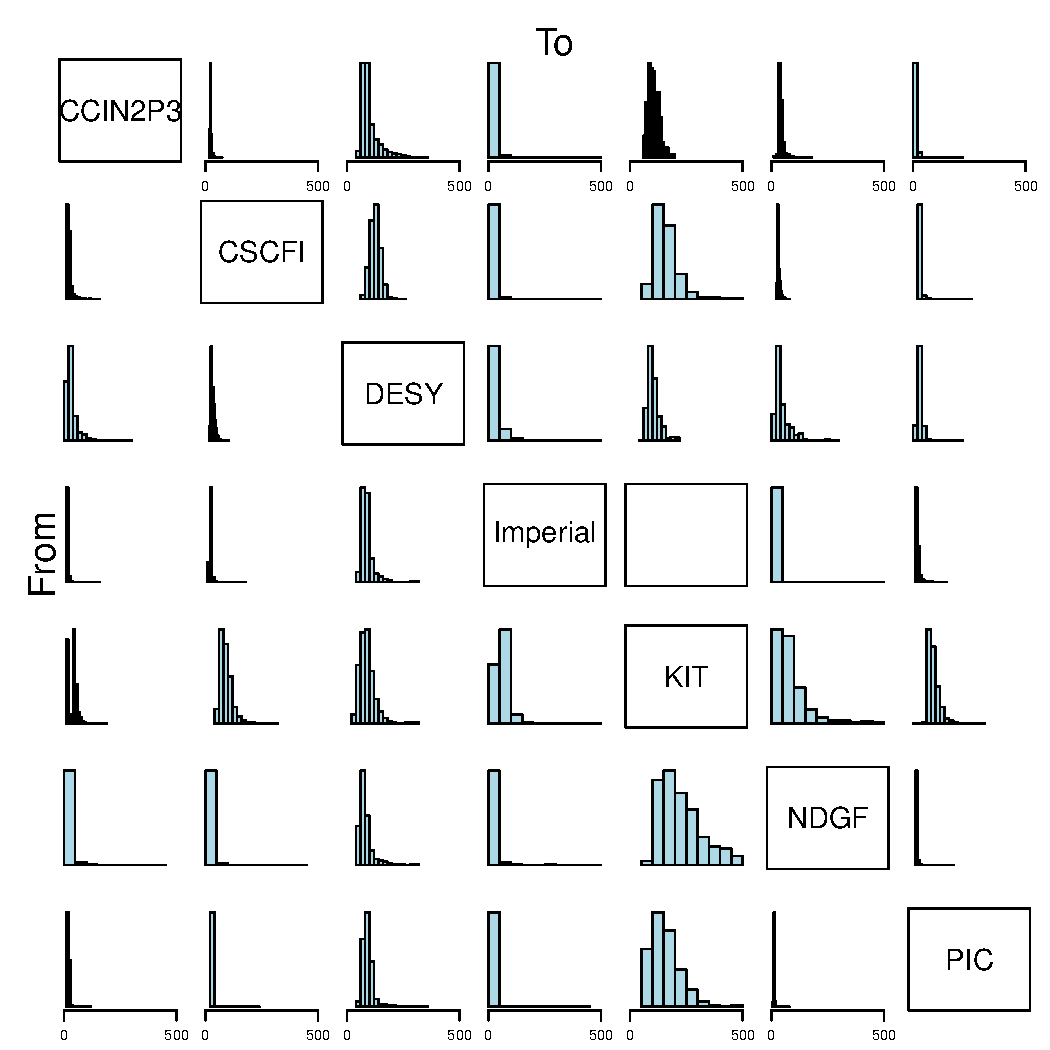
\includegraphics[width=0.8\textwidth]{fts3-mesh.pdf}
       \caption{The FTS3 transfer testbed. Rows show transfers from the named site, columns show transfers to the destination. The horizontal axis for all plots is fixed at 500 seconds, i.e. transfers that proceed at less than 2 MB/sec will overflow.}
 \label{fig:fts3-mesh}
\end{figure}


\subsection{FTS3 server and dCache SE at KIT}
For managing file transfers between sites, an FTS3 instance is setup at KIT. Furthermore, a storage element based on dCache 2.10 on Scientic Linux is created. Both instances are rolled out on physical machines.

\subsubsection{FTS3}
FTS3 supports IPv6 in its baseline version. The service has to be bind to IPv6 locally in the FTS3 conguration (IP=::) and to be enabled explicitely for gfal2 ( IPV6=true). The host is available in the DNS as default dual-host, with IP4 and IPv6 announced in the A and AAAA records, and also with IPv4-only or IPv6-only names with an -ipv4 or -ipv6 appendix, respectively. Thus, all aliases have to included in the host certicate.

File transfers are successfully brokered by the FTS3 instance via IPv4 and IPv6 between the sites. Since most FTS3 instances in production use a separated database instance for performance and failsafe reasons, moving the database to a dedicated machine was tested as well. For the SQL db backends supported by FTS3, IPv6 support had been implemented in MySQL v5.5.3 and MariaDB v5.5.35, which are not available in the baseline SL6 repositories. MariaDB was installed on a dedicated host with version 5.5.42. After binding mysql locally to IPv6 as well ([mysqld] bind-address = ::), the database could be connected remotely with an IPv6-ready mysql client. For the FTS3 service to connect to the remote database via IPv6, the address has to be escaped explicitly, i.e., encapsulating the IP as [IP6]:PORT/fts3 and may depend on the version of the database library used by the FTS3 service.

\subsubsection{dCache based SE}
A dCache instance is setup on a dedicated host. The main hurdle for file transfer access was a reverse lookup by the instance when receiving a file request. After explicitely setting the dual-stack, IPv4-only, and IPv6-only host names in the dCache congfiguration (srm.net.local-hosts=hostname-ipv4,ipv6) and the general hosts file, the storage element is accessible via IPv4 and IPv6 as well.


\section{IPv6 readiness of storage technology for WLCG}
\subsection{Storage technology}

For the FTS3-based testbed SRM \cite{SRM2.2} was selected as more production-like 
than the old gridftp-based one. 

All sites participating selected dCache, as it had matured into the only full-stack storage 
system to fully support dualstack and IPv6-only setups.

\subsubsection{Protocol: SRM}

SRM is built on SOAP which in turn is built on HTTP. It's designed to be protocol-independent as it only sends data in one stream and only processes TURLs and SURLs.
It's however only used to set up the transfer, and the real transfer is handled by other protocols.

\subsubsection{Protocol: HTTP}

Transfer over HTTP or HTTPS work without problems for reads, but the implementations for writing are differing between different software leading to limited usability.
It is used in production for reads at some sites, most notably NDGF-T1.

\subsubsection{Protocol: GSIFTP} 

GSIFTP or GridFTP\cite{GFTP1.0} is FTP with an extra layer on top for multistreaming and autentication. It's currently widely used with SRM, but has issues with IPv6 since it sends the IP address of where to
connect to instead of using hostnames. All current servers and clients break the GridFTP-2.0 document \cite{GFTP2.0} in the same way to support "Delayed Passive", a method for redirecting writes from the client directly to the storage without a multihost storage environment like dCache having to proxy the write. 


\subsubsection{Protocol: XROOTD} 

XROOTD by SLAC is a general purpose random-IO protocol for data access. It supports IPv6 from release 4.0.0.


\subsubsection{Software: dCache} 

dCache is a Java-based software for building distributed storage solutions. It supports many different access protocols and authentication methods.

\subsubsection{Software: DPM} 

DPM or Disk Pool Manager was the software used by many sites for the previous testbed. It 


\section{IPv6 perfSONAR measurements}
%\section{IPv6 perfSONAR measurements}

The WLCG has adopted the perfSONAR toolkit \cite{perfsonar} for
the monitoring of its network infrastructure and this project is
being coordinated by the WLCG Network and Transfer Metrics group
\cite{wlcg-NTMG}.  The WLCG perfSONAR configuration system operates around
groups of sites with a common purpose and these are known as meshes.
For example, there are meshes for each WLCG country
group (e.g. UK, DE, FR etc.) or experiment such as USATLAS or USCMS or
network groupings such as LHCONE and LHCOPN. Until recently testing
between members of the groups was configured using JSON files held on a
web-server at CERN specifying the group members and test parameters. A
site administrator configuring a perfSONAR host for a mesh needed to add
the URL of the JSON file corresponding to that mesh into a configuration
file on the perfSONAR host. This worked but required effort from all
site administrators involved. The mesh configuration system has recently
undergone development. This is described in detail in \cite{wlcg-NTMG},
but briefly, the system has evolved from the use of the manually
configured JSON files to a more automated system which is significantly
easier to configure. Each perfSONAR host now has a so-called auto-mesh
URL e.g. \\{\tt\small  
https://myosg.grid.iu.edu/pfmesh/mine/hostname/psum01.aglt2.org}\\
containing configuration details for the meshes that the perfSONAR host
has been added to. The meshes are maintained using a mesh-configuration
GUI provided by the US Open Sciences Grid (OSG) using data collected
from both the GOCDB and OSG Information Management System (OIM). The
perfSONAR toolkit has the ability to monitor both IPv4 and IPv6 network
connectivity. Consequently, in addition to the meshes mentioned above, we
have added a mesh containing perfSONAR hosts known to have both IPv4 and
IPv6 connectivity, i.e. a dual-stack mesh. The mesh tests throughput and
latency between hosts over both IPv4 and IPv6. Results are available from
the web sites of the relevant perfSONAR hosts, for example the perfSONAR
bandwidth host at WLCG site UKI-SOUTHGRID-OX-HEP at the University of
Oxford: \\{\tt\small http://t2ps-bandwidth.physics.ox.ac.uk/toolkit/}\\ 


\section{Status of LHCOPNv6/LHCONEv6}
\subsection{LHCOPN/LHCONE}
Based on the actions initiated at Grid Deployment Board in November and December 2014, to request tier-1s to join the HEPiX-IPv6 working group and to encourage sites moving their production endpoints to dual stack even if this requires concessions of the quotation of their site relatability and site availability. The proposal of the LHC experiment Atlas was to
\begin{itemize}
 \item request that all Tier-1s provide,
	besides an IPv6 peering to LHCOPN,
        a dual stack PerfSONAR machine by first of April 2015
 \item request that Tier-2s provide,
        besides an IPv6 peering to their LHCONE connection,
        a dual stack PerfSONAR machine by August 2015.
\end{itemize}
At the last LHC[OPN/ONE] meeting a proposal was put forward to the effect that
LHCOPN connecting Tier-1 sites to CERN would get IPv6-ready by 1. April 2015 and
LHCONE connecting Tier-[123] sites would become IPv6 ready by August 2015.
No objections to this proposal were presented. The following Tier-1 sites are actively announcing an IPv6 peering to LHCOPN: CH-CERN, DE-KIT, ES-PIC, FR-CCIN2P3, NDGF, NL-T1. IT-INFN-CNAF is currently preparing the IPv6 peering. The group of IPv6 peers over LHCONE is currently even smaller: besides CH-CERN this are the two sites CEA SACLAY and FR-CCIN2P3.
The ipv6 peerings are reflected at the PerfSONAR dualstack dashboard url:\\
{\tt\small http://maddash.aglt2.org/maddash-webui/index.cgi?dashboard=Dual-Stack\%20Mesh\%20Config}\\. It implies that there are still some LHC tier-1 sites, more than two month after the agreed deadline, not offering ipv6 cidr via their LHCONE peering.


\section{Outlook and future plans}
The HEPiX IPv6 working group has made good progress during the last 18 months. It has been demonstrated that access 
to remote dual-stack federated data storage services in a production-like environment functions well with FTS, SRM and dCache.
During the remainder of 2015 tests on other storage technologies will be performed. Members of the group will deploy dual-stack services
on more production instances of storage services and other essential central services to enable the proper measurement of 
data transfer performance over IPv6 and to 
demonstrate to the experiments and the WLCG management that it is safe to migrate to dual-stack. The deployment of IPv6 peering on 
LHCOPN/LHCONE and dual-stack perfSONAR instances will be tracked and encouraged. Both of these are pre-requisites to the wider deployment
of production dual-stack services. In parallel with these activities the group also aims to provide more training sessions and guidance
on best practice in the management of IPv6 services and site operations. Once there are a sufficient number of dual-stack services 
deployed on WLCG it will be possible to support the use of IPv6-only clients within the production infrastructure.


\par
\section*{References}

\begin{thebibliography}{1}
\bibitem{ipv6wg} {\tt http://hepix-ipv6.web.cern.ch}
\bibitem{rfc} All Internet Engineering Task Force Requests For Comments (RFC) documents are available
from URLs such as http://www.ietf.org/rfc/rfcNNNN.txt where NNNN is the RFC number, for example {\tt http://www.ietf.org/rfc/rfc2460.txt}
\bibitem{ipv6stat} See for instance {\tt http://www.google.com/ipv6/statistics.html}. The 2\% global connectivity threshold was crossed in September 2013.
\bibitem{rhel} {\tt http://www.redhat.com/products/enterprise-linux/}
\bibitem{cream}
Aiftimiei C, Andreetto P, Bertocco S, Dalla Fina S, Dorigo A,
Frizziero E, Gianelle A, Marzolla M, Mazzucato M, Sgaravatto M,
Traldi S, Zangrando L 2010 Design and Implementation of the gLite CREAM Job
Management Service {\it Future Generation Computer Systems} Volume {\bf 26} Issue
4 pp 654-667, doi: 10.1016/j.future.2009.12.006.
\bibitem{wms}
Cecchi M, Capannini F, Dorigo A, Ghiselli A, Giacomini F, Maraschini M, Marzolla M, Monforte S, Pacini F, Petronzio L, Prelz F 2009 The gLite Workload Management System {\it Advances in Grid and Pervasive Computing: 4th International Conference, GPC}
\bibitem{panda}
Maeno T 2008 PanDA: distributed production and distributed analysis
system for ATLAS {\it J. Phys. Conf. Ser.} {\bf 119} 062036
\bibitem{fts}
Kunszt P, Badino P, Rocha R, Casey J, Frohner A, McCance G 2006 The gLite File Transfer Service
{\it Workshop on Next Generation Distributed Data Management at The Fifteenth IEEE International Symposium on High-Performance Distributed Computing (HPDC2006), Paris, France}
\bibitem{phedgen}
Egeland R, Metson S and  Wildish T 2008 Data transfer infrastructure for
CMS data taking,  {\it XII Advanced Computing and Analysis Techniques in
Physics Research (Erice, Italy: Proceedings of Science)}
\bibitem{cvmfs}
Blomer J et al 2012 Status and future perspectives of CernVM-FS
{\it J. Phys.: Conf. Ser.} {\bf}396 052013
\bibitem{bdii}
Field L and Schulz M W 2004  Grid Deployment Experiences: The path to a production quality LDAP based grid information system {\it Proceedings of the International Conference on Computing in High Energy and Nuclear Physics (CHEP 2004)}
\bibitem{monalisa}
Legrand I, Newman H, Voicu R, Cirstoiu C, Grigoras C, Dobre C, Muraru A,
Costan A, Dediu M and Stratan C 2009 MonALISA: An agent based, dynamic
service system to monitor, control and optimize distributed systems {\it
Computer Physics Communications} Volume {\bf180} Issue 12, December 2009,
Pages 2472–2498
\bibitem{LifeCycle}
    Wildish T 2013 Integration and validation testing for PhEDEx, DBS and DAS with the PhEDEx LifeCycle agent {\it also presented at CHEP 2013}
\bibitem{cms}
The CMS Collaboration 2008 The CMS experiment at the CERN LHC {\it JINST
{\bf 3} S08004}
\bibitem{PhEDEx}
    Egeland R, Wildish T, Metson S 2008 Data transfer infrastructure for CMS data taking {\it XII Advanced Computing and Analysis Techniques in Physics Research (Erice, Italy: Proceedings of Science)}
\bibitem{FTS3}
    Salichos M, Keeble O, Alvarez Ayllon A, Kamil Simon M 2013 FTS3 - Robust, simplified and high-performance data movement service for WLCG {\it also presented at CHEP 2013}
\end{thebibliography}


\end{document}

